\section{Computação Gráfica e Modelagem 3D}
%%------------------------------------------------Introducao--------------------------------------------------------%%%%
A computação gráfica esta presente em quase tudo na vida do homem, desde de pequenos jogos para celular até projetos grandiosos para viagens espaciais, tendo também um papel importante na medicina, onde possibilita a visualizações de órgãos internos ao corpo humano o que vem ajudando no tratamento de várias doenças\cite{comp_grafica_h}\cite{azevedo}\cite{kirne}. Esta presente também em muitos outros segmentos, tais como os descritos na Tabela~\ref{tab:comp_teoria}. \\

\begin{table}
\centering
\begin{tabular}{|l|l|}
	\hline
	Área & Aplicações \\ \hline
	Medicina &  Exames, diagnósticos, estudo, planejamento de procedimentos\\ \hline
	Arquitetura & Perspectivas, projetos de interiores e paisagismo\\ \hline
	Engenharia & Em todas as suas áreas (mecânica, civil, aeronáutica etc.)\\ \hline
	Meteorologia & Previsão do tempo, reconhecimento de poluição\\ \hline
	Segurança Pública & Definição de estratégias, treinamento, reconhecimento\\ \hline
	Astronomia & Tratamento de imagens, modelagem de superfícies\\ \hline
	Artes & Efeitos especiais, modelagens criativas, esculturas e pinturas\\
	\hline
\end{tabular}
\caption{Diferentes ramos da computação gráfica.}
\label{tab:comp_teoria}
\end{table}

Um dos pioneiros nesse ramo da computação foi o aluno do \textbf{MIT}, \textit{Ivan Sutherland}, que criou um programa de desenho chamado Sketchpad\cite{sutherland}. Onde usando uma caneta a laser podia-se desenha na tela de um computador, salvar e depois recarregar o desenho feito.\\

O primeiro computador com recursos gráficos de visualização de dados numéricos foi o \textbf{Whirlwind I}, também desenvolvido pelo \textbf{MIT}. Utilizado primeiramente pelas industrias automobilística e aeroespacial, ele foi se desenvolvendo, alavancando a computação gráfica a um patamar de grande visibilidade, assim fazendo com que ela evoluisse de forma surpreendente.\cite{comp_grafica_h2}.\\

%%%%%%%%%%%%%%%%%%%%%%%%%%%%%%%%%%%%%%%%%%%%%%%%%%%%%%%%%%%%%%%%%%%%%%%%%%%%%%%%%%%%%%%%%%%%%%%%%%%%%%%%%%%%%%%%%%%%%%%%%%%%%%%%%%%%%%%%%%%
%%------------------------------------------------------Fim-Introducao-----------------------------------------------------------------%%%%
%%%%%%%%%%%%%%%%%%%%%%%%%%%%%%%%%%%%%%%%%%%%%%%%%%%%%%%%%%%%%%%%%%%%%%%%%%%%%%%%%%%%%%%%%%%%%%%%%%%%%%%%%%%%%%%%%%%%%%%%%%%%%%%%%%%%%%%%%%%

\subsection{Sistemas de Coordenadas}
Um sistema de coordenada é aquele que se utiliza para descrever objetos modelados em um universo. Através dele consegue-se capturar a posição e as dimensões dos objetos. Existem vários sistemas, a Figura~\ref{fg:coordenadas} mostra três deles, que são: coordenadas polares, esféricas e cilíndricas. O primeiro deles é dado por um raio e um ângulo. Já no segundo sistema, obtemos as coordenadas pelo raio e dois ângulos. No terceiro, consegue-se um ponto qualquer na região de análise através de um raio, um ângulo e um comprimento.\\ 

\begin{figure}[ht!]
	\centering
	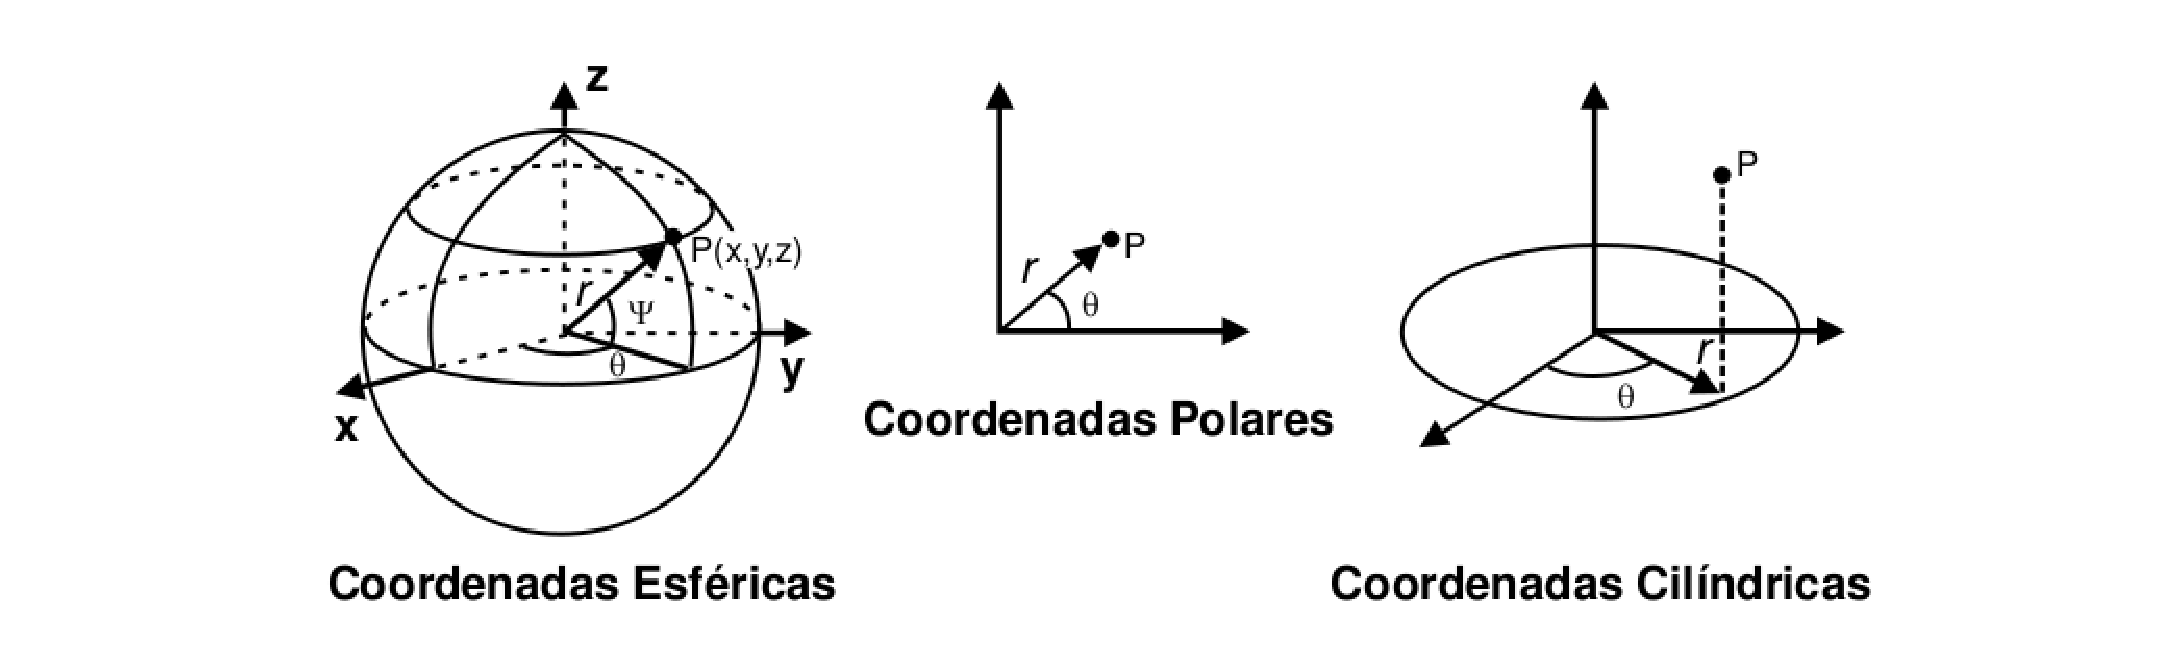
\includegraphics[scale=0.4]{s_coordenadas}
	\caption{Sistemas de coordenadas.}
	\label{fg:coordenadas}
\end{figure}

\subsection{Transformações}
As transformações são umas das características mais importantes da computação gráfica. Elas representam um mapeamento de ponto(s) de uma determinada posição para outra~\cite{comp_grafica1}. As transformações mais usadas e conhecidas são: rotação, escala e translação.\\

%%%%%%%%%%%%%%%%%%%%%%%%--------------tranlasao---------------%%%%%%%%%%%%%%%%%%%%%%%%%%
Transladar significa mover o objeto. Essa operação é dada pela equação~\ref{eq:translacao}, onde adicionando quantias($T_x$, $T_y$ e $T_z$) a sua coordenada atual($x$, $y$ e $z$), obtém-se uma nova posição, transladada($x'$, $y'$ e $z'$). A Figura~\ref{fg:trans} ilustra essa transformação. \\

\begin{equation}\label{eq:translacao}
[x'\ y'\ z'] = [x\ y\ z] + [T_{x}\ T_{y}\ T_{z}]
\end{equation}

\begin{figure}[ht!]
	\centering
	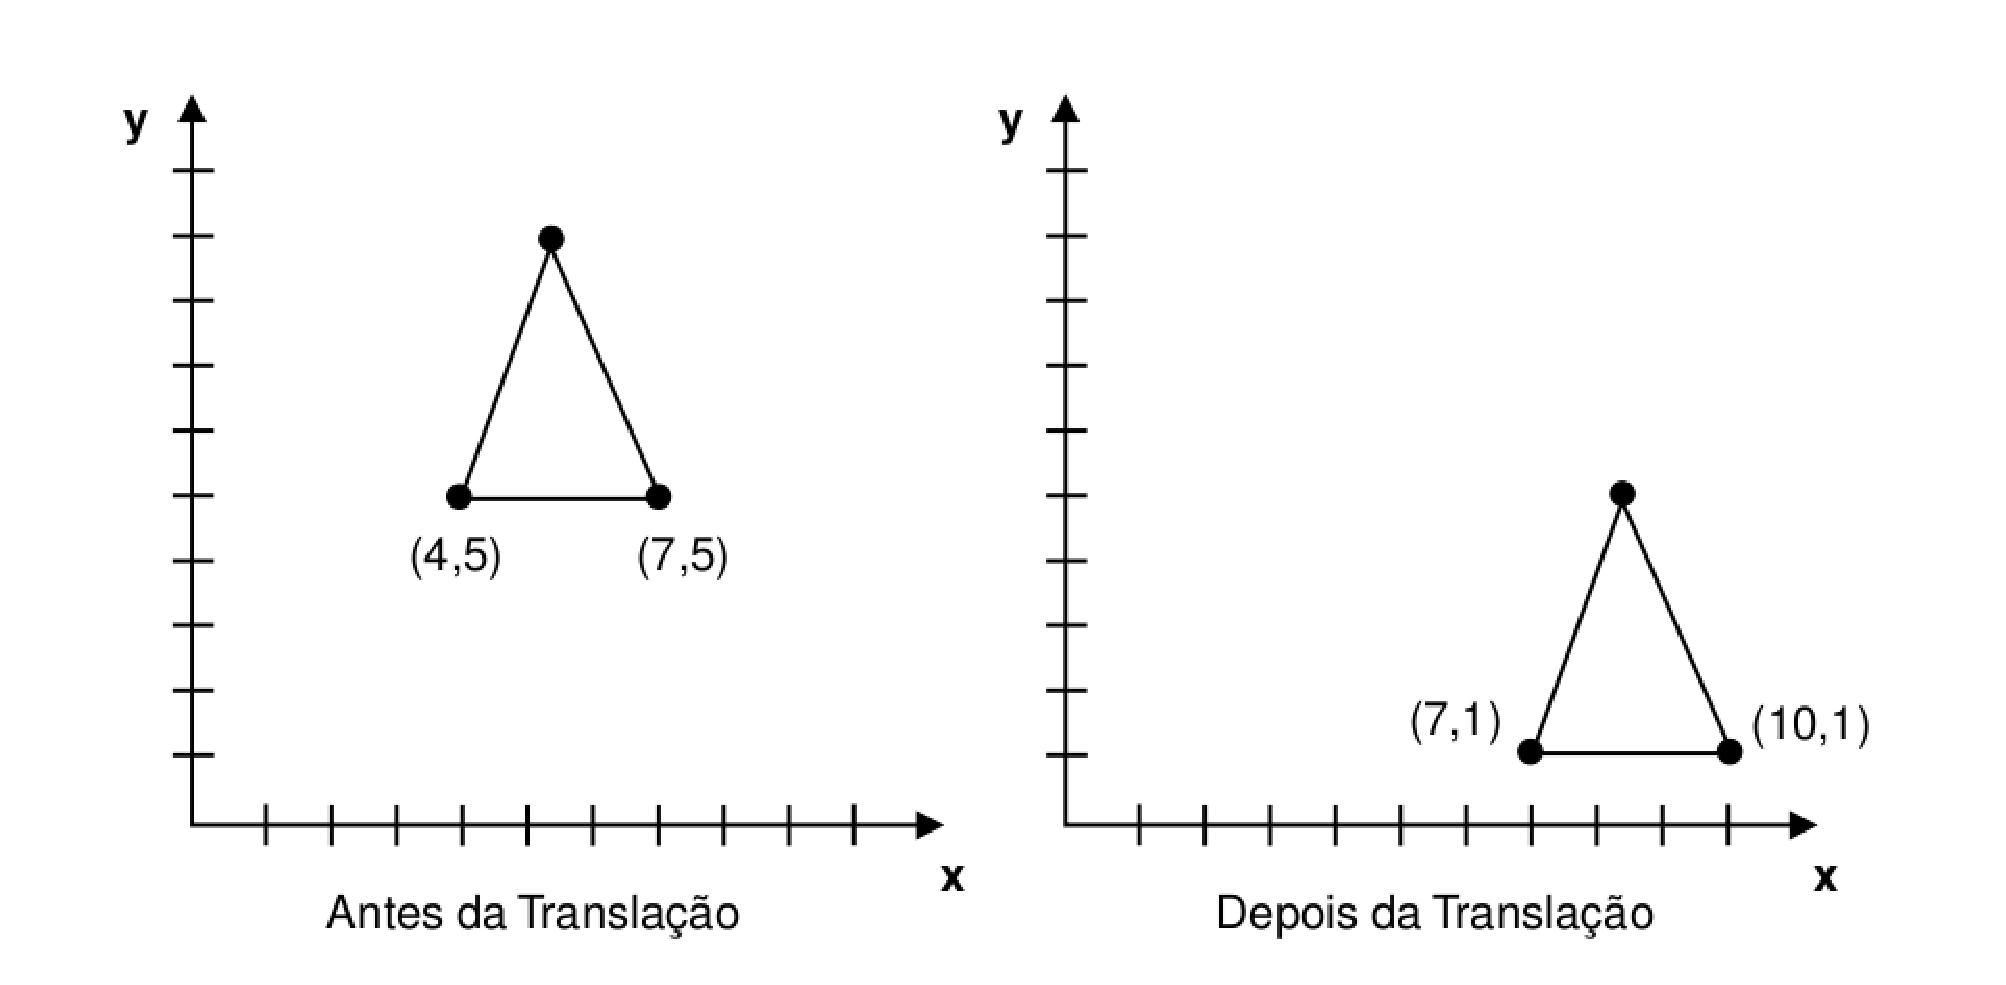
\includegraphics[scale=0.4]{trans}
	\caption{Operação de Translação 2D.}
	\label{fg:trans}
\end{figure} 

%%%%%%%%%%%%%%%%%%%%%--------------escala---------------%%%%%%%%%%%%%%%%%%%%%%%%%%%%%%%
A operação de escala é aquela associada à mudança de dimensão dos objetos. Ela é representada pela equação matricial~\ref{eq:escala}, que mostra que quando multiplicamos as dimensões atuais ($x$, $y$ e $z$) por alguns fatores ($S_x$, $S_y$ e $S_z$), obtemos um novo objeto escalado ($x'$, $y'$ e $z'$). A Figura~\ref{fg:escala} mostra bem o que ocorre quando escalonamos um objeto.\\

\begin{equation}\label{eq:escala}
    \begin{array}{c c c}
    [x' \ y' \ z'] = [x \ y \ z]
    \begin{bmatrix}
     S_x & 0 & 0   \\[0.2em]
     0 & S_y & 0   \\[0.2em]
     0 & 0 & S_z
    \end{bmatrix}
    \
    = [xS_x\ yS_y\ zS_z]
    \end{array}
\end{equation}

\begin{figure}[ht!]
      \centering
	  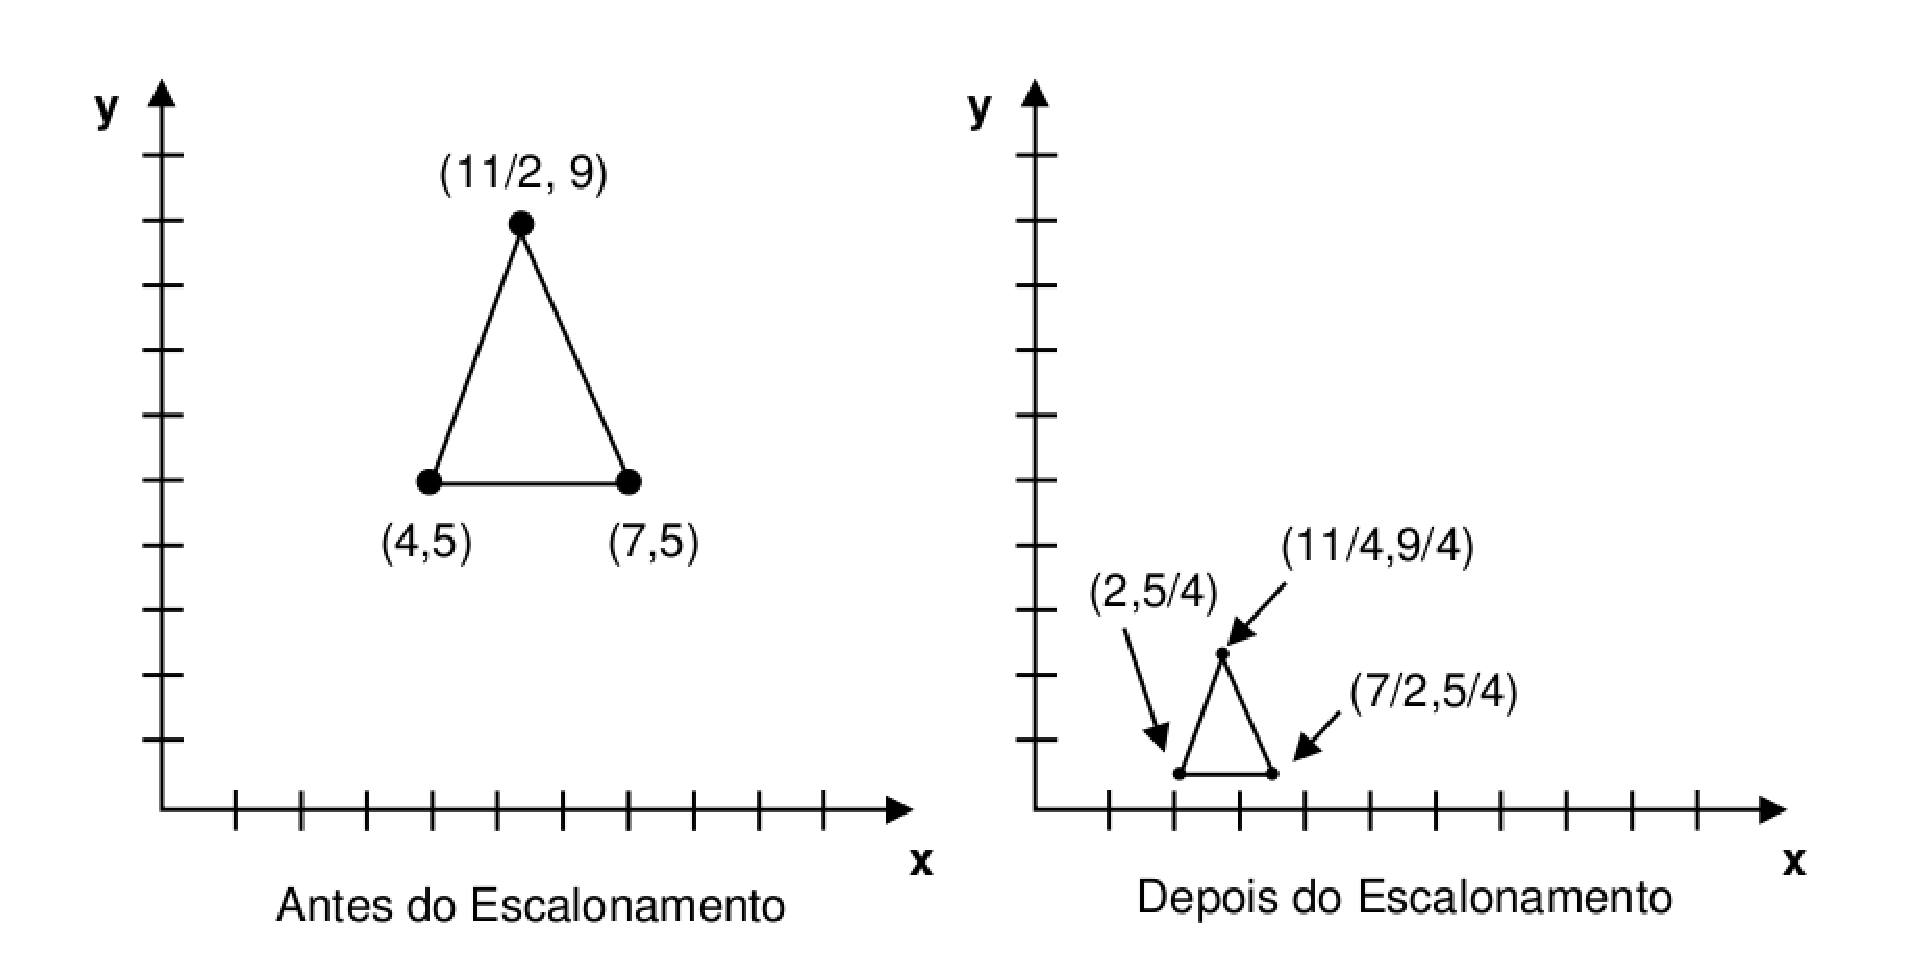
\includegraphics[scale=0.4]{escala}
	  \caption{Operação de Escala 2D.}
	  \label{fg:escala}
\end{figure} 

%--------------rotacao---------------
Por fim, quando desejamos girar um objeto ou um ponto no nosso sistema de coordenadas, usamos a transformação de rotação, a qual pode ser representada pelas formas matriciais~\ref{eq:rotacao}, que mostram, respectivamente, as matrizes rotação para os eixos $x$, $y$ e $z$. A Figura~\ref{fg:rotacao}, ilustra essa operação.

\begin{figure}[ht!]
      \centering
	  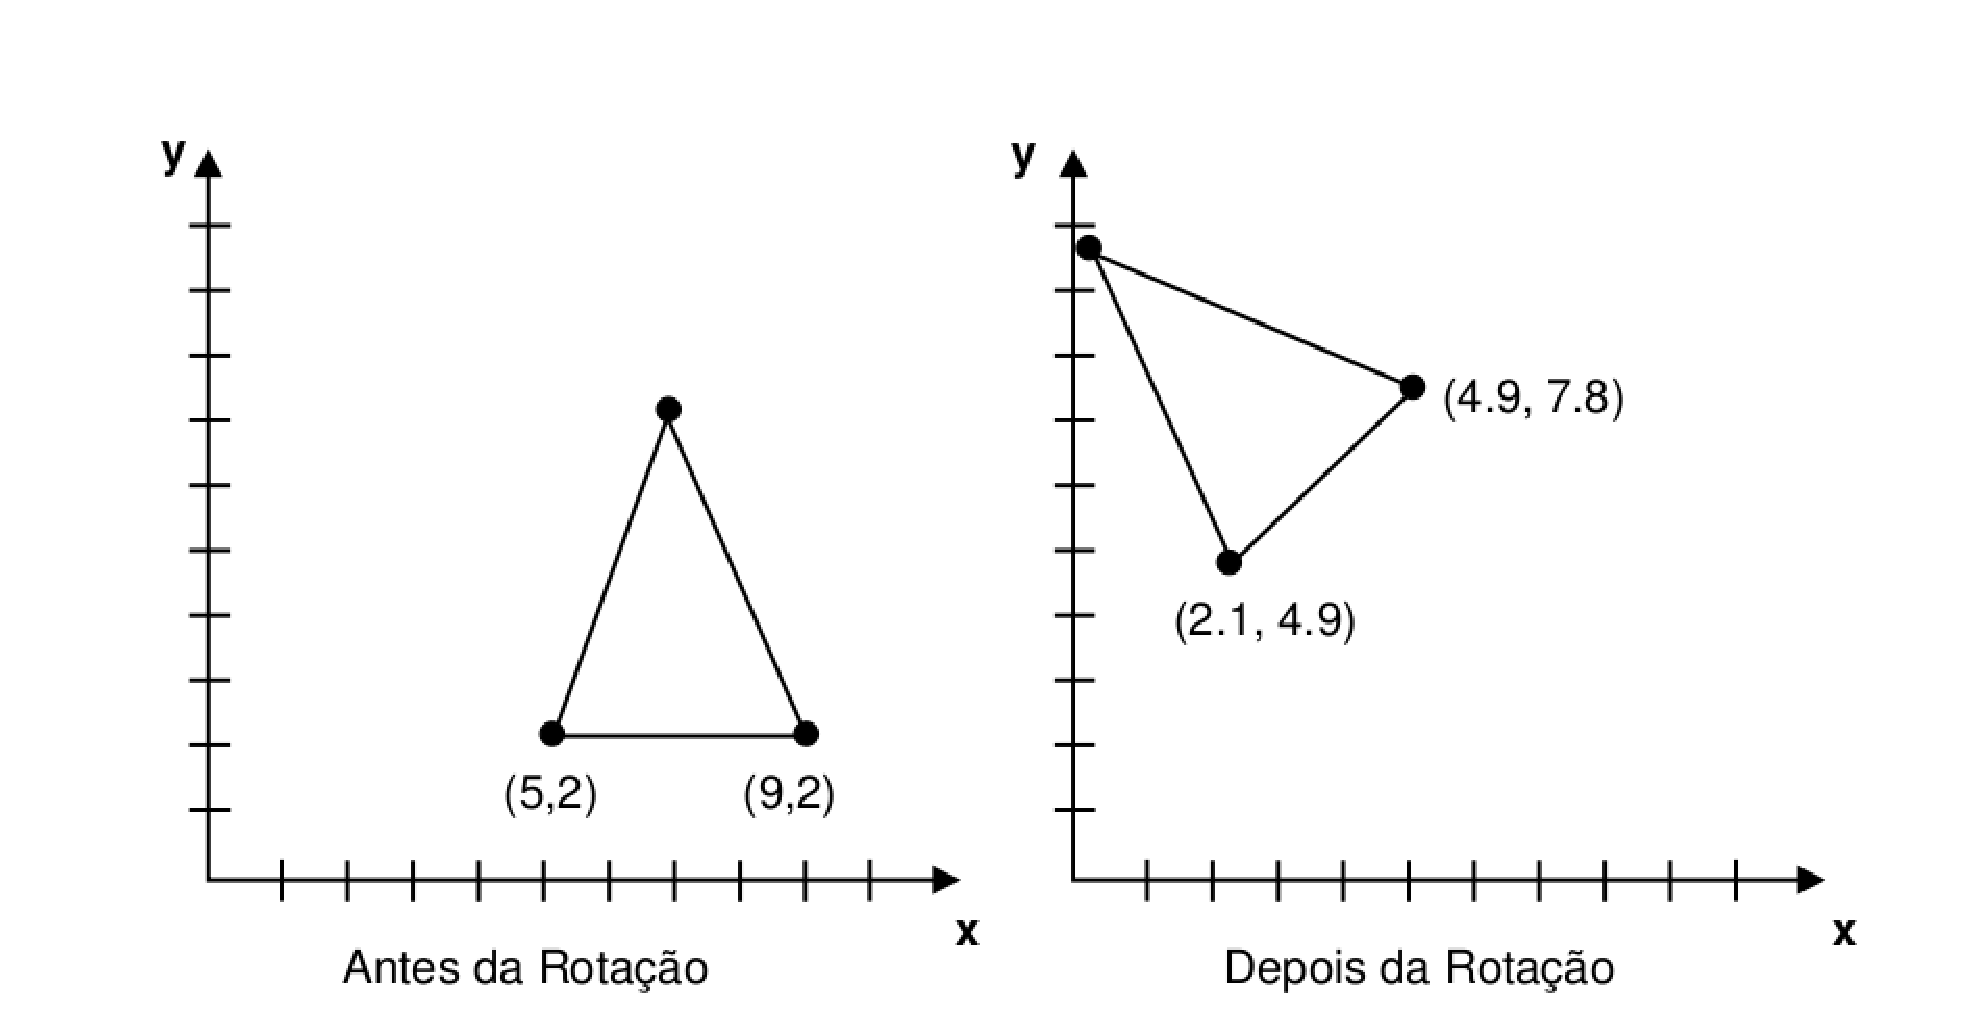
\includegraphics[scale=0.4]{rotacao}
	  \caption{Operação de Rotação 2D.}
	  \label{fg:rotacao}
\end{figure} 
\begin{center}
\begin{equation}\label{eq:rotacao}
  \begin{array}{c c c}
     R_x(\theta) = \begin{bmatrix}
    1 & 0 & 0   \\[0.2em]
    0 & \cos(\theta) & -\sin(\theta)    \\[0.2em]
    0 & \sin(\theta) & \cos(\theta) \\
    \end{bmatrix}
    , 
    R_y(\theta) = \begin{bmatrix}
    \cos(\theta) & 0 & \sin(\theta) \\[0.2em]
    0 & 1 & 0   \\[0.2em]
    -\sin(\theta) & 0 & \cos(\theta)\\
    \end{bmatrix}
    ,
    R_z(\theta) = \begin{bmatrix}
    \cos(\theta) & -\sin(\theta) & 0\\[0.2em]
    \sin(\theta) & \cos(\theta) & 0\\[0.2em]
    0 & 0 & 1\\\ 
    \end{bmatrix}
    \end{array}
\end{equation}
\end{center}

\subsection{Representação de Sólidos}
\subsubsection{Representação Armada ou Wireframe}
É a representação dada por um conjunto de arrestas que define as bordas do objeto\cite{speck}. Tem a vantagem de ser mais rápida quanto a renderização, porém tem um problema relacionado ao fato de dar margem para várias interpretações, além de dificultar cálculos como: volume e massa de sólidos. Por isso, ela geralmente não é considerada uma técnica de modelagem de sólidos. A Figura~\ref{fg:wireframe} esta ilustrando essa técnica.

\begin{figure}[ht!]
	\centering
	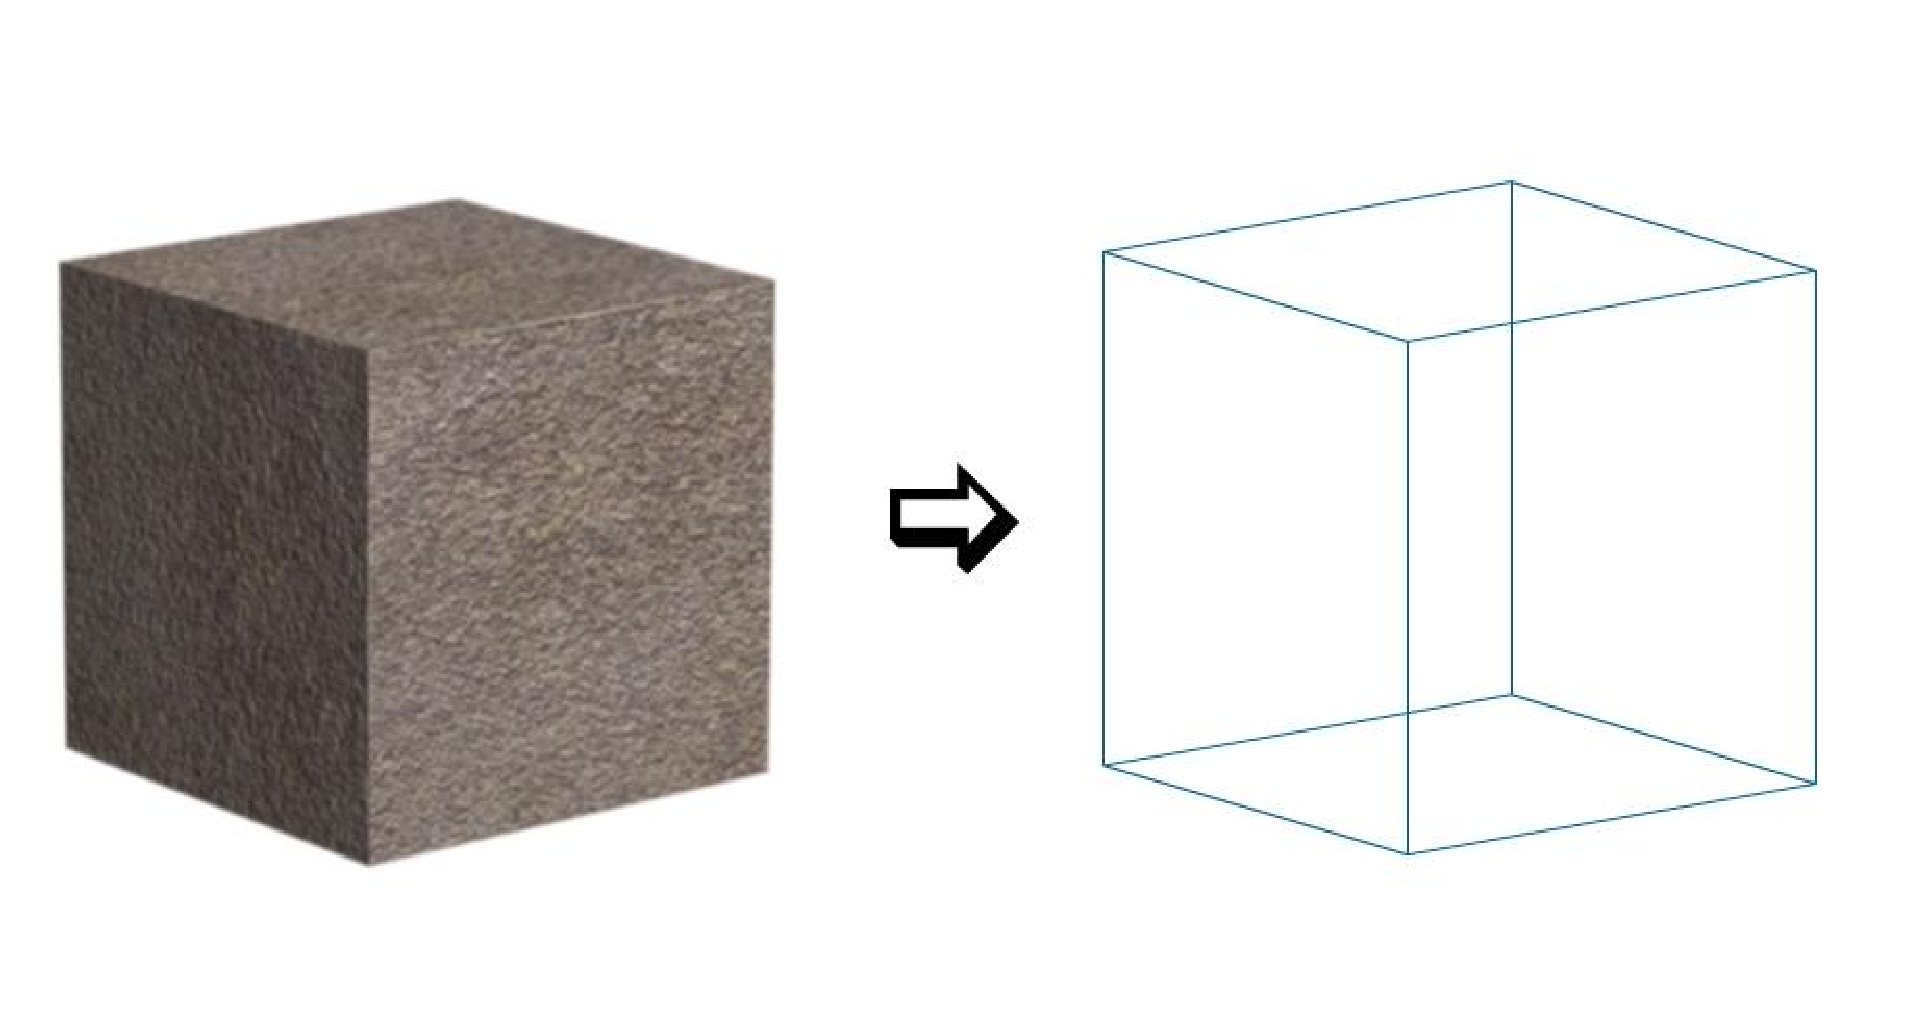
\includegraphics[scale=0.2]{wireframe}
	\caption{Representação Armada ou Wireframe.}
	\label{fg:wireframe}
\end{figure} 

\subsubsection{Representação por Faces} 
\label{sec:r_faces}
Usa faces delimitantes que descrevem os contornos do sólido. É uma das formas mais usuais na modelagem de objetos tridimensionais nos dias de hoje. Ela  também é conhecida com  \textbf{Boundary Representation} ou \textbf{B-rep}, que consiste na descrição de  objetos pelos seus contornos, ou seja, arestas e vértices. Para melhor entendimento, temos a Figura~\ref{fg:faces} como exemplo dessa representação.

\begin{figure}[ht!]
      \centering
	  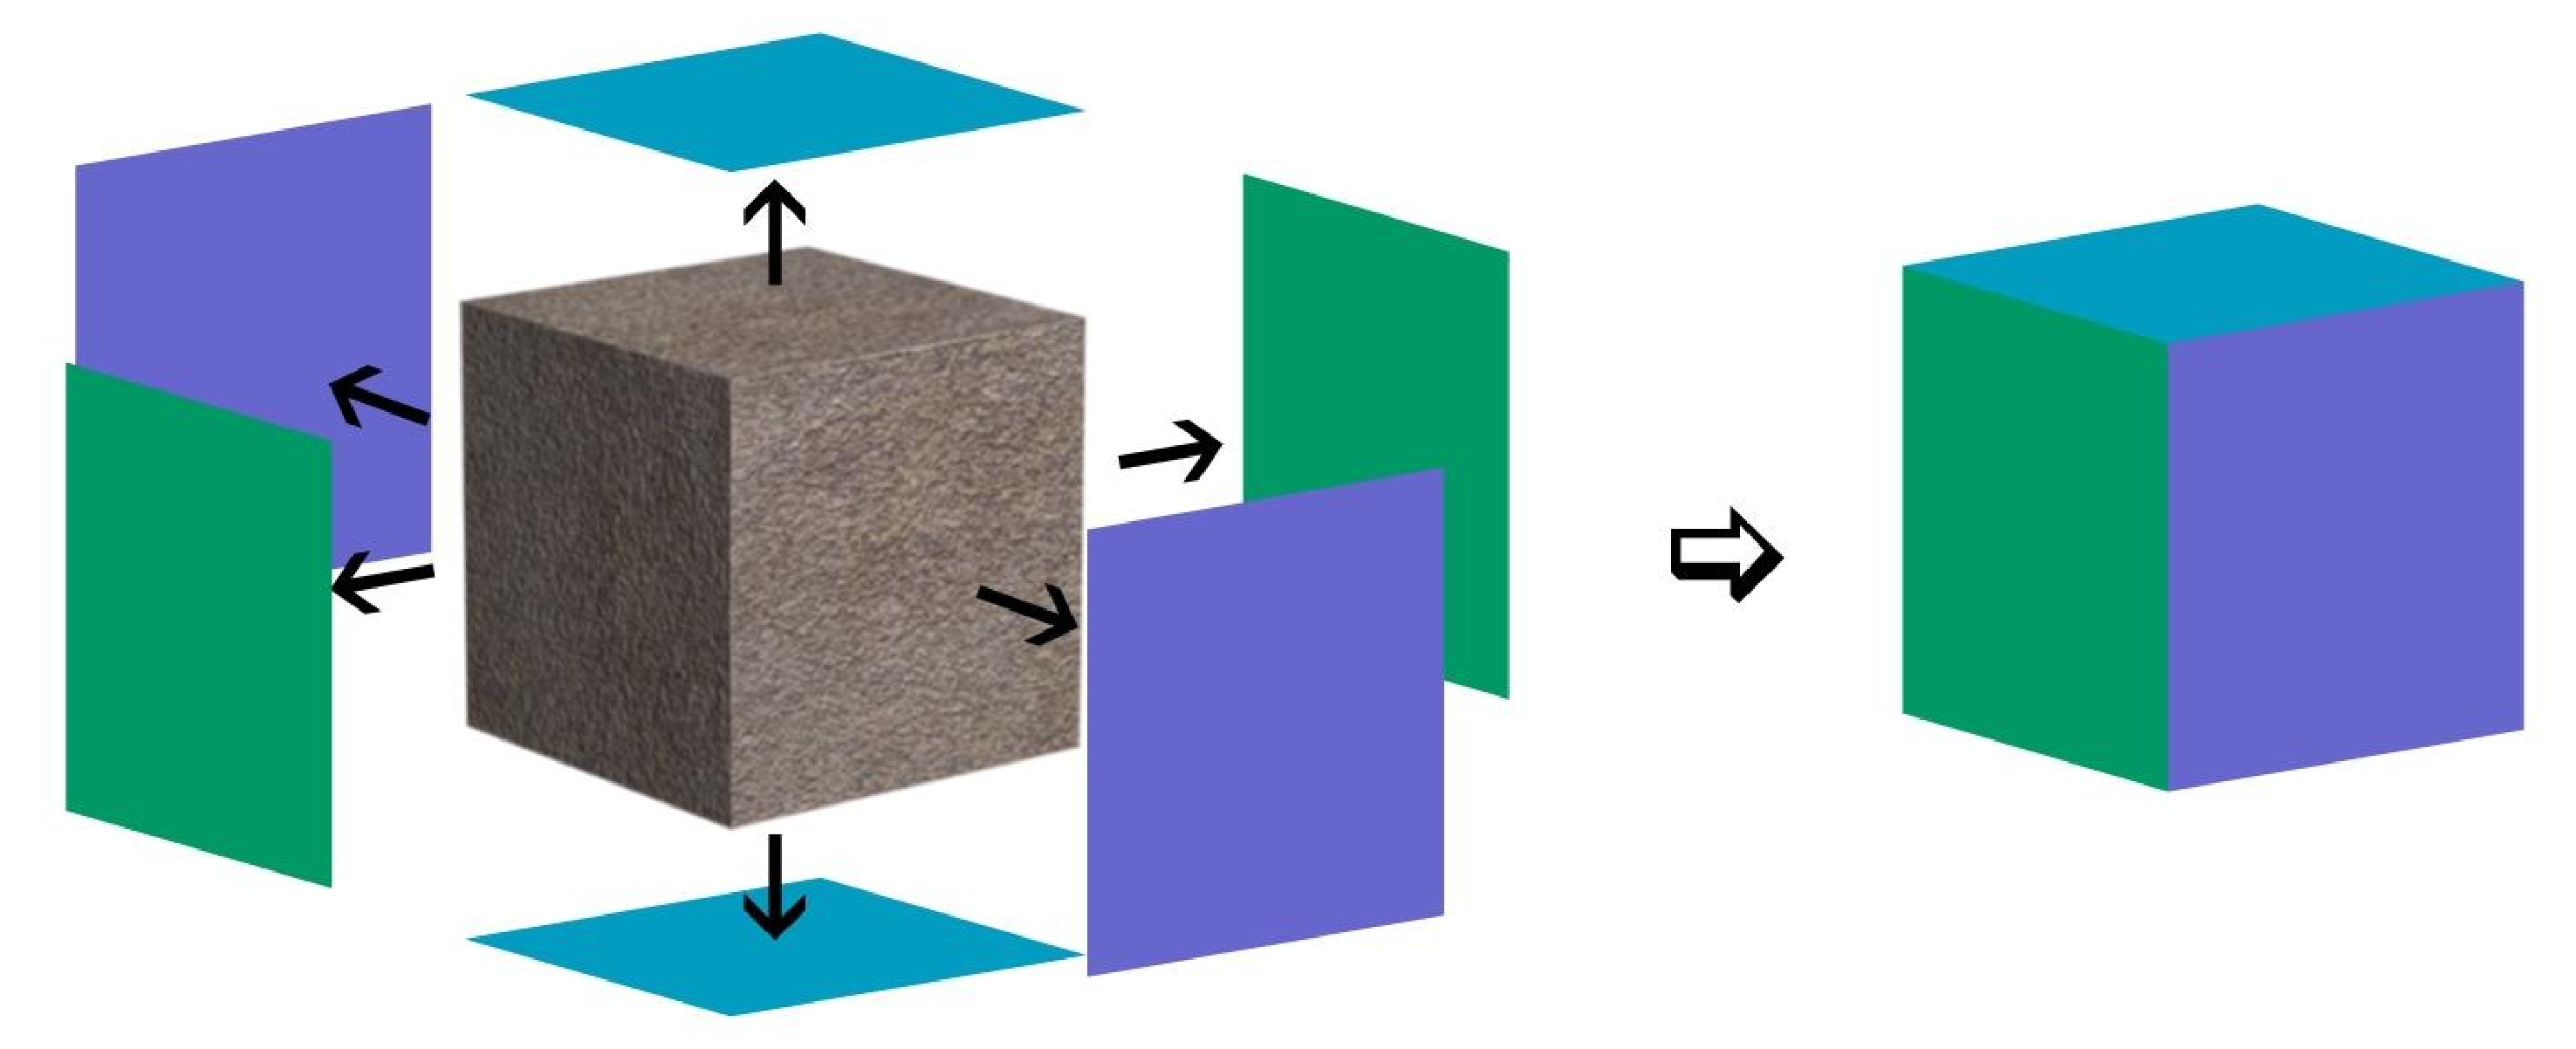
\includegraphics[scale=0.2]{faces}
	  \caption{Representação por Faces.}
	  \label{fg:faces}
\end{figure} 

\subsubsection{Representação Poligonal}
Polígono vem do grego \textit{polys}, que significa muitos, e \textit{gonos} que significa ângulos, assim esse representação é formada por figuras planas com muitos seguimentos de reta e muitos ângulos. Então podemos construir sólidos com o polígono mais simples, o triângulo, até um mais complexo, com um número elevado de lados(Figura~\ref{fg:pilogono}). Essa técnica pode ser considerada uma especificação do caso apresentado na seção~\ref{sec:r_faces}.\\

\textit{Tesselation} é um das características dessa representação, significa preencher uma dada região através de várias repetições de um mesmo polígono até não haver mais espaços em "branco". A maioria das máquinas de jogos utilizam a representação por faces triangulares. Isso se deve ao fato de esta necessitar de menos processamento e também por possibilitar a representação de qualquer tipo de contorno\cite{traina}.

\begin{figure}[ht!]
      \centering
	  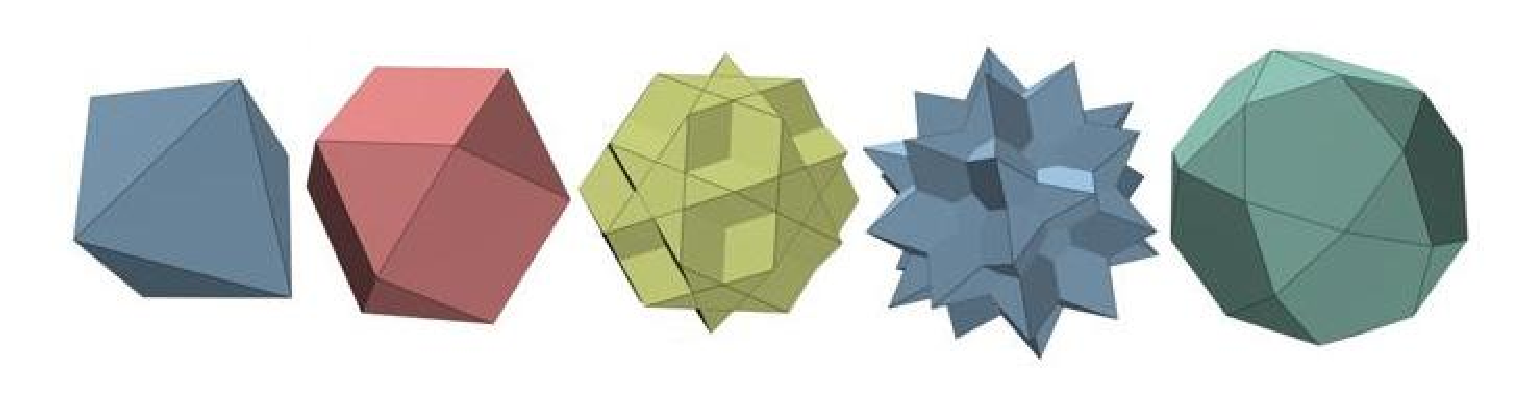
\includegraphics[scale=0.2]{poligonos}
	  \caption{Representação Poligonal.}
	  \label{fg:pilogono}
\end{figure} 

\subsection{Técnicas de Modelagem Geométrica}
Quanto ao âmbito da modelagem de objetos tridimensionais, tem-se basicamente três categorias: a manual, matemática e automática. \\

O método manual foi a base de toda a modelagem atual. É a técnica mais barata e mais antiga.  Utiliza-se basicamente das medidas do modelo real e, é claro, da habilidade do modelador. Já à matemática utiliza de algoritmos para gerar o objeto desejado. Esse método é muito utilizado para modelar, por exemplo, a proliferação de organismos microscópicos.\\

Modelagem automática é o método mais recente. Utiliza-se de scanners muitos sofisticados para obter o modelo tridimensional de qualquer ambiente ou sólido.

\subsubsection{Combinação de Objetos}
É um dos métodos mais intuitivos e antigos. É realizado através da combinação de um ou mais sólidos básico para obtenção de um outro\cite{hearn}, mostrado na Figura~\ref{fg:comb}. O  único detalhe que deve-se prestar bastante atenção nessa técnica, é a questão das operações booleanas(interseção, união e subtração) em alguns casos não gerarem como resultado um sólido, por exemplo, no caso da intercessão de dois cubos que não estão em contato, temos como resultado o vazio que não é um sólido válido.

\begin{figure}[ht!]
	\centering
	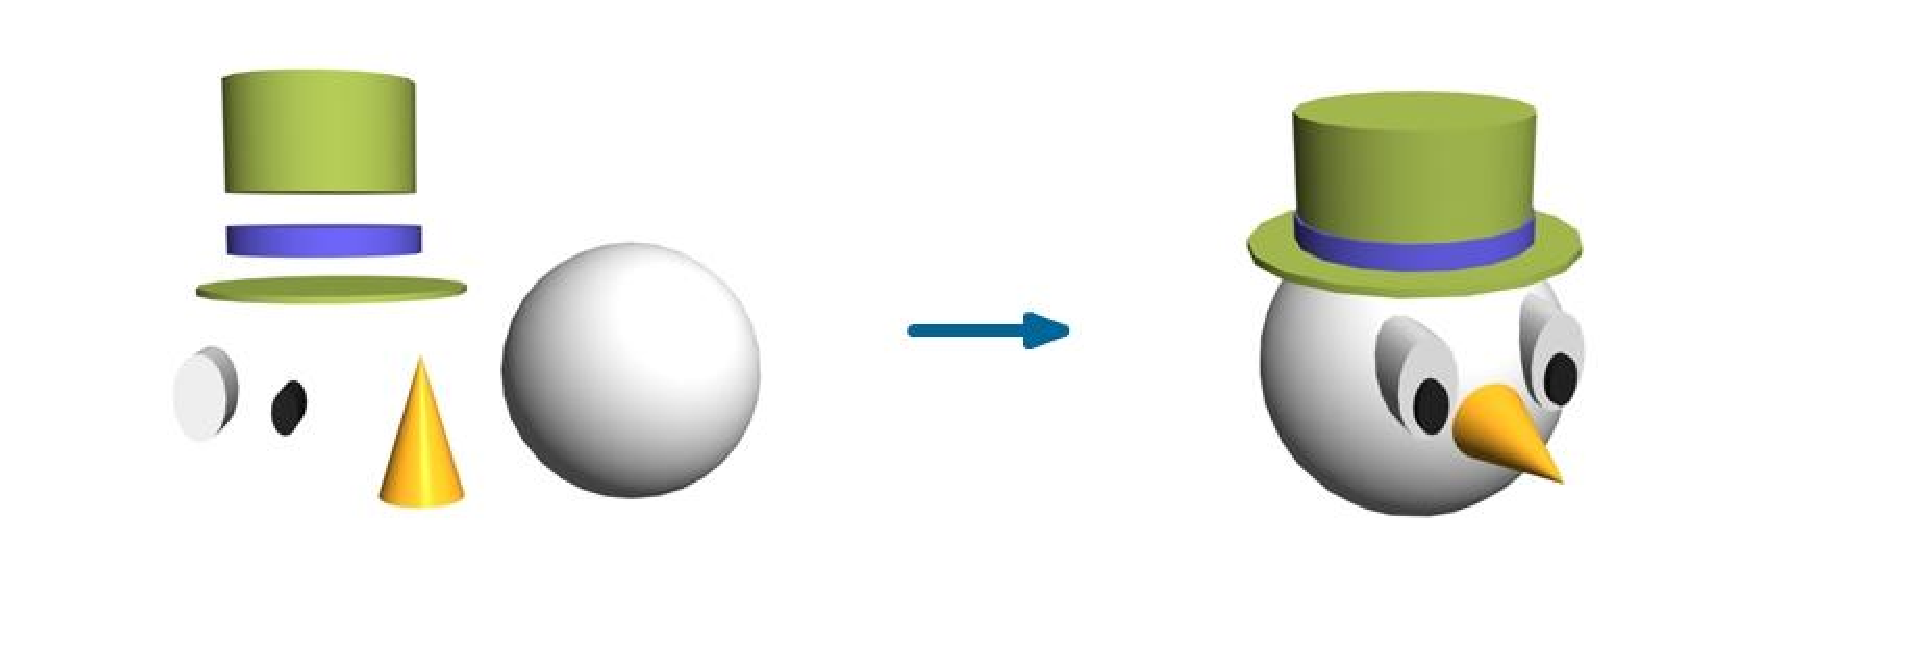
\includegraphics[scale=0.4]{montagem}
	\caption{Modelagem por Combinação de Objetos.}
	\label{fg:comb}
\end{figure} 

\subsubsection{Modelagem por Varredura(Sweep)}
A modelagem por varredura é obtida pela movimentação de uma curva $N_1$ na trajetória de uma outra curva $N_2$ que descreverá um superfície que poderá ser usada como sólido. Sendo $N_1$ nomeada de \textit{Curva de Contorno} e $N_2$ de \textit{Caminho ou Diretriz}\cite{3dsmod}.\\

Ainda no questão da varredura, pode-se sitar dois casos particulares que são: varredura por \textit{Extrusão}(Figura~\ref{fg:etrusao}) ou \textit{Translacional}(Figura~\ref{fg:rotacional}) e a \textit{Rotacional}. Para o a primeira é a translação de uma superfície na forma circular, por exemplo , ao longo de uma direção, gerando um sólido(no caso um cilindro). No segundo caso ocorre a rotação de uma superfície ao longo de um eixo ou ponto de referência, resultando também em um sólido.

\begin{figure}[ht!]
	\centering
	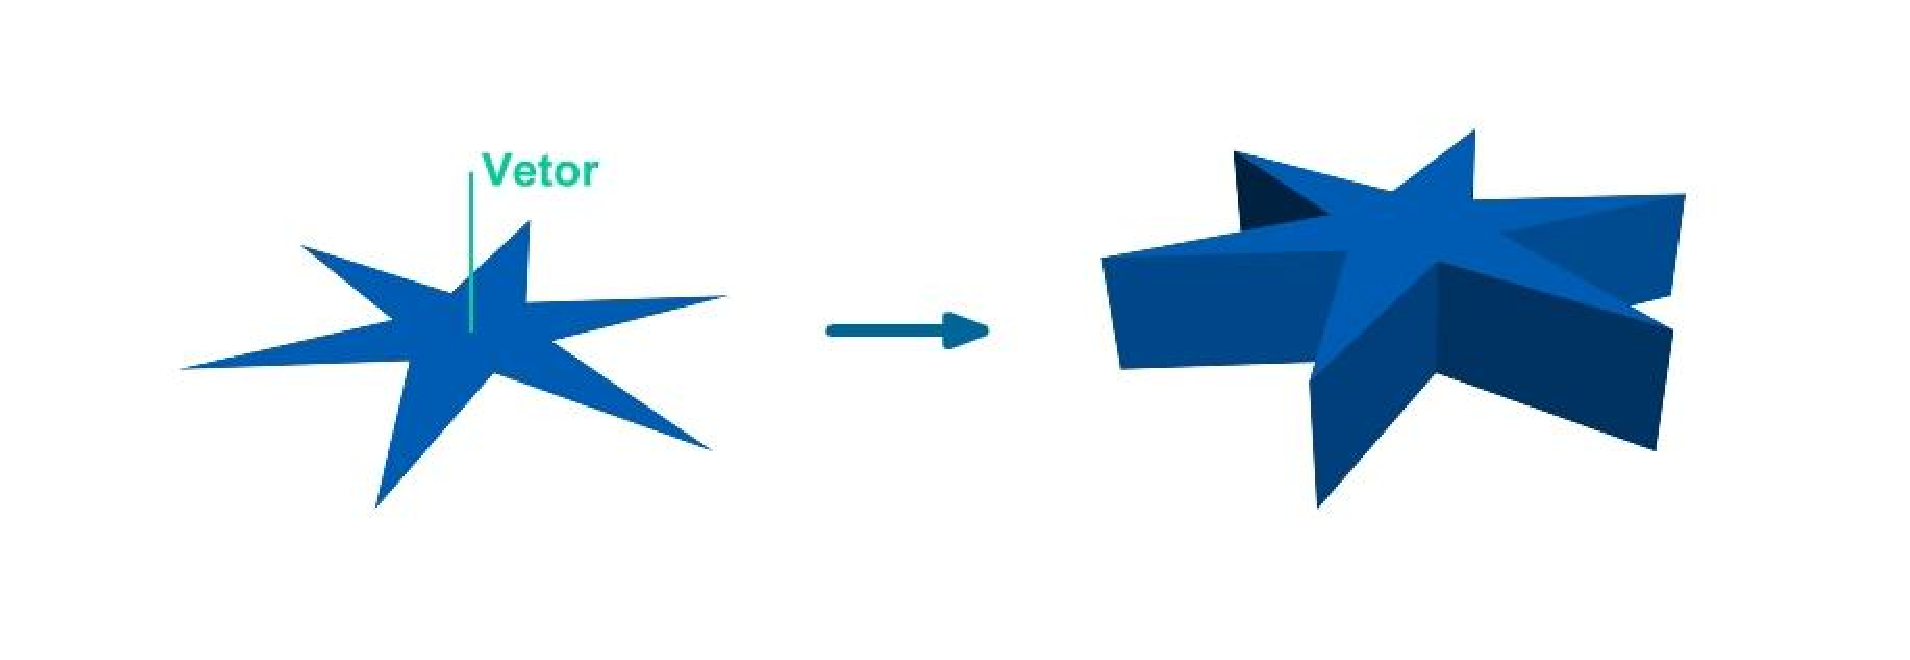
\includegraphics[scale=0.4]{extrude}
	\caption{Modelagem por Extrusão.}
	\label{fg:etrusao}
\end{figure} 
\begin{figure}[ht!]
	\centering
	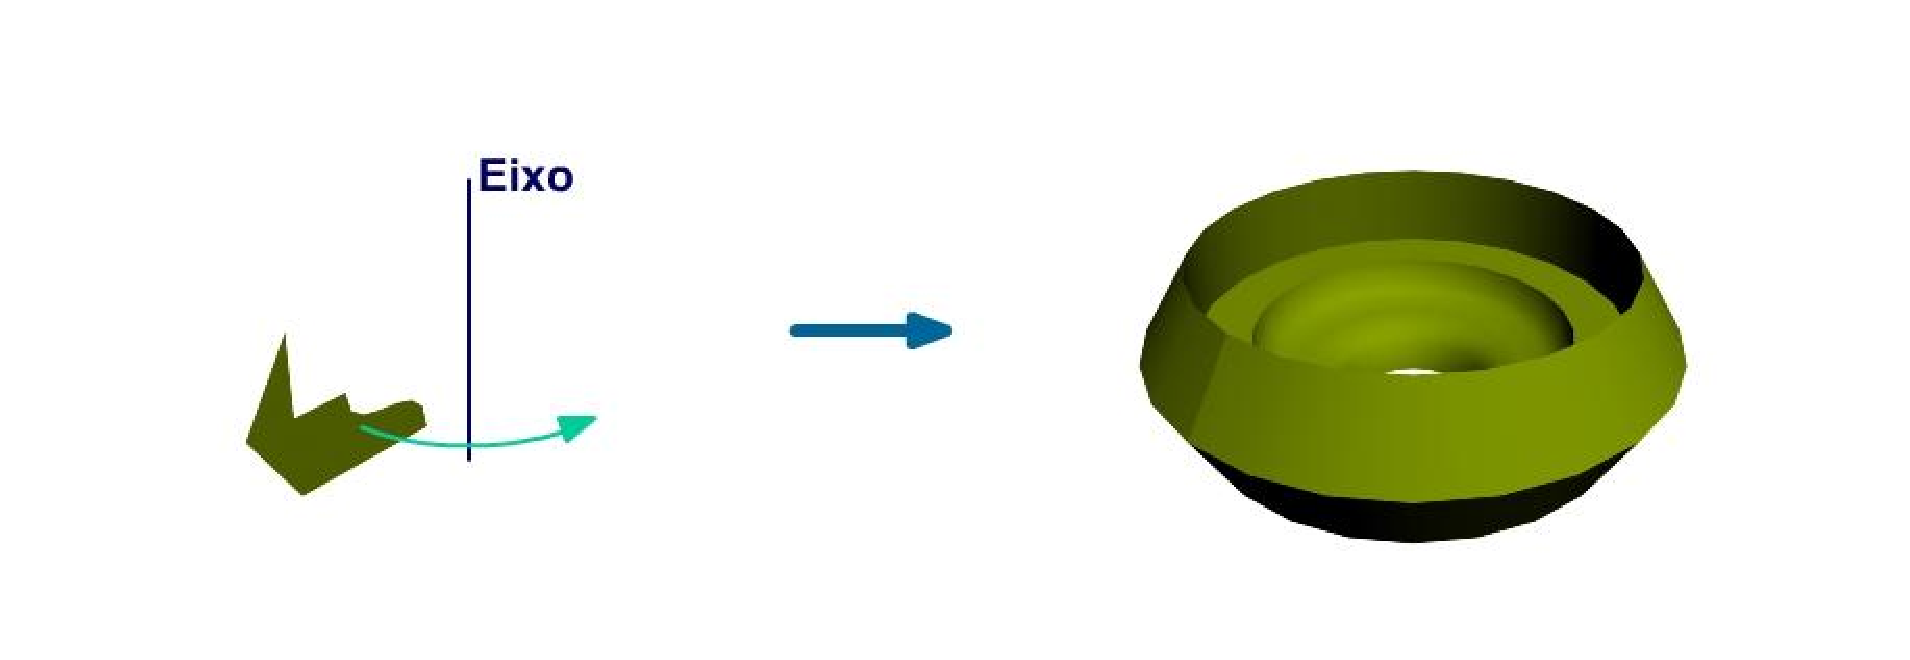
\includegraphics[scale=0.4]{rotacional}
	\caption{Modelagem Rotacional.}
	\label{fg:rotacional}
\end{figure} 

\subsection{Realidade Virtual}
O termo Realidade Virtual surgiu na década de 80 pelo artista e cientistas da computação, Jaron Lanier, que uniu os dois universos, que até então eram, muito distantes, o mundo real e o virtual\cite{jane}. Porém há registro de trabalhos anteriores a essa denominação, dentre eles esta o primeiro capacete que permitia imersão, e também pode-se falar do famoso SENSORAMA\cite{rhen}(que não obteve um grande sucesso comercial, pelo seu valor, mas com certeza foi um dos trabalhos que deram impulso para o futuro dos ambientes virtuais).\\

Mas o que é Realidade Virtual? É uma interface avançada que permite o usuário, navegar, modificar, interagir em tempo real com uma determinada aplicação. Existem basicamente dois tipos de realidade virtual quanto o fator imersão a imersiva e a não imersiva. A primeira é caraterizada por permitir ao usuário se sentir dentro do ambiente(através do uso de capacetes especiais, óculos, luvas, roupas, caves~\cite{cave}, sensores, entre outros dispositivos), já a segunda isso não ocorre(onde usa-se mouse, teclado, monitores , etc)\cite{aect}.

\subsubsection{Grafo de Cena}
É um dos conceitos mais importantes da teoria de jogos, e também da computação gráfica. Sua definição é a de ferramenta para representação de ambientes virtuais tridimensionais. Sendo esse ambiente descrito por diversos aspectos, dentre eles: descrição geométrica, câmera, transformação, aparência, comportamento e iluminação\cite{ferreira}. O cenário é formado por todos esses aspectos inseridos dentro do grafo de cena. \\

O grafo de cena é formado por nós, compondo arrestas que tem como resultado um grafo acíclico direcionado. Com cada nó tendo atributos ,sitados anteriormente, que poderão ou não influenciar nos outros nós que estão conectados a ele. Existe uma classificação para eles, que os divide em três categorias: nós raiz(é o primeiro nó, no qual todos os outros estão ligados de forma direta ou não) ,nós internos (geralmente contem informações de transformações 3D - rotação, escala e translação) e por fim estão os nós folha(que por padrão contem as dados de representação geométrica dos objetos da cena).\\ 

A propriedade fundamental dessa ferramenta é o que se chama de herança de estado. Que diz que cada nó deve herda as propriedades de estado do seus ancestrais até o nó raiz. Então se tivermos um grafo de cena formado por um \textit{nó} raiz, casa, e dois \textit{nós folha}, sendo o primeiro uma cadeira e o segundo mesa. Se rotacionarmos o \textit{nó} casa, por consequência teremos a cadeira e a mesa rotacionadas também. Porém no caso da rotação de um dos \textit{nós folha}, o \textit{nó} casa permanecerá inalterado, haja vista que ele esta hierarquicamente no nível acima e a cadeira também não se moverá pelo fato de ter uma ligação direta com esse nó(esta no mesmo nível e não tem conexão direta). Na tabela~\ref{tb:grafo_cena} estão algumas vantagens proporcionadas pelo uso dessa técnica.\\

\begin{table}
\centering
\begin{tabular}{|p{3cm}|p{8cm}|}
	\hline
	\multicolumn{2}{|c|}{Vantagens} \\ \hline
	Produtividade &  Gerencia e reduz o numero de linhas que seriam necessárias para implementar
a mesma funcionalidade utilizando uma interface de baixo nível, como a OpenGL.\\ \hline
	Portabilidade &  Encapsula todas as tarefas de baixo nível, reduzindo e até 
excluindo a parte de código que é especifica de uma plataforma.\\ \hline
	Escalabilidade &  Possibilita trabalhar tanto em máquinas com configurações básicas até supercomputadores.\\ 
	\hline
\end{tabular}
\caption{Vantagens proporcionadas pelo uso do grafo de cena.}
\label{tb:grafo_cena}
\end{table}

\section{Irrlicht}
O Irrlicht é uma máquina de jogo de alta performasse escrita em linguagem C++\cite{irrlichtbook}. Contem todas as característica que pode-se encontrar em qualquer outra \textit{engine}\footnote{Máquina de jogo.}. Existem muitos projetos desenvolvidos e em desenvolvimento usando-a, com uma boa comunidade, onde pode-se tirar dúvidas e publicar trabalhos e melhorias. E além de tudo isso, é completamente livre\cite{irrlicht}.\\

Ela tem como principais características:
\begin{enumerate}
\item Renderização em tempo real de alta performasse usando \textbf{Direct3D} e \textbf{OpenGL}.
\item Independe de plataforma.
\item Renderiza diretamente de arquivos, tais como : .zip, .pak, .pk3, etc.
\item Rápida e fácil detecção de colisão.
\item Possibilita o uso de vários linguagens de programação, como : Java, Delphi, entre outras.
\item Limpa, fácil de entender, e bem documentada.
\end{enumerate}

\section{Método FDTD}
O termo Método FDTD(Finite-Differene Time-Domain Method), primeiramente chamado de como Algorítimo de Yee, foi criado por Kane Yee em 1966\cite{yeebook}. É uma técnica capaz de solucionar, de forma simples e elegante, numericamente as equações de Maxwell, de maneira direta. Tem como características principais: 1)distribuição geométrica discreta das componentes de campos Elétrico e Magnético em células, de maneira a satisfazer tanto a Lei de Faraday quanto a Lei de Ampère nas formas diferencial e integral e 2)aproximação das derivadas espaciais e temporais por diferenças finitas, de forma a se obterem equações explicitas para a atualização temporal de todas as componentes de campo\cite{rodrigo}.\\

Porém, por algum tempo, esse método foi deixado de lado devido ao fato de ter um custo computacional muito alto, aliado a isso, deve-se levar em consideração o contexto histórico em que ele se encontrava, onde os computadores ainda eram bem limitados. Mas, um tempo depois, ressurgiu através dos trabalhos de dois cientistas, chamados Allen e Brodwin, que aplicaram essa técnica para problemas tridimensionais relacionados à interação eletromagnética com meios materiais\cite{allen}. Assim, novas técnicas apareceram e melhoram a abordagem do método, acompanhado , é claro, da evolução dos computadores.\\

Essa técnica tem sido usada desde então, em uma grande quantidade de aplicações, entre elas estão: radares, antenas, fotônica, sistemas de telecomunicação, medicina, estruturas periódicas, sistemas de aterramento, entre várias outras.\\

O método FDTD aplicado com intuito de simular uma propagação eletromagnética, utiliza as equações de Maxwell na forma diferencial.
\begin{equation}\label{eq:faraday}
	\overline{\nabla}\times\overline{E}=-\mu\frac{\partial \overline{H}}{\partial t},
\end{equation}
\begin{equation}\label{eq:ampere}
		\overline{\nabla}\times\overline{H}=\epsilon\frac{\partial \overline{E}}{\partial t} + \overline{J},
\end{equation}
		
	Onde:\\
	$\overline{J} = \sigma\overline{E}$, vetor densidade de corrente elétrica  de condução(ampere/$m^{2}$).\\ 

As equações (\ref{eq:faraday}) e (\ref{eq:ampere}) expandidas em coordenadas retangulares, geram as respectivas equações escalares, mostradas abaixo.
\begin{equation}
	\frac{\partial H_x}{\partial t} = \frac{1}{\mu}(\frac{\partial E_y}{\partial z}-\frac{\partial E_z}{\partial y}),
\end{equation}
\begin{equation}
	\frac{\partial H_y}{\partial t} = \frac{1}{\mu}(\frac{\partial E_z}{\partial x}-\frac{\partial E_x}{\partial z}),
\end{equation}
\begin{equation}
	\frac{\partial H_z}{\partial t} = \frac{1}{\mu}(\frac{\partial E_x}{\partial y}-\frac{\partial E_y}{\partial x}),
\end{equation}

\begin{equation}
	\frac{\partial E_x}{\partial t} = \frac{1}{\epsilon}(\frac{\partial H_z}{\partial y}-\frac{\partial H_y}{\partial z} -\sigma E_x),
\end{equation}
\begin{equation}
	\frac{\partial E_y}{\partial t} = \frac{1}{\epsilon}(\frac{\partial H_x}{\partial z}-\frac{\partial H_z}{\partial x} -\sigma E_y),
\end{equation}
\begin{equation}
	\frac{\partial E_z}{\partial t} = \frac{1}{\epsilon}(\frac{\partial H_y}{\partial x}-\frac{\partial H_x}{\partial y} -\sigma E_z)
\end{equation}

sendo:\\
$E_x, E_y, E_z$ e $H_x, H_y, H_z$ representam as componentes dos campos elétrico $\overline{E}$ e magnético $\overline{H}$, respectivamente. Essas componentes são funções do tempo $t$ e das três coordenadas cartesianas ($x,y,z$).\\

A lei de Faraday, equação (\ref{eq:faraday}), informa que quando há variação no tempo do vetor $\overline{B}=\mu\overline{H}$ (vetor densidade de fluxo magnético, em teslas), surgem componentes de campo elétrico circulando em torno da(s) componente(s) deste vetor. Já a lei de Ampère, equação (\ref{eq:ampere}), informa que quando há variação no tempo do vetor $\overline{D}=\epsilon\overline{E}$ (vetor densidade de fluxo elétrico, em ) em certa direção e/ou a presença da fonte de corrente $\overline{J}$, esta causa circulação de campo magnético em torno da direção da(s) componente(s) deste vetor.\\
			
Kane Yee se baseou nessa duas observações para definir seu esquema  de distribuição espacial  e temporal das componentes  de campo  de seu algoritmo. Sua representação geométrica, chamada de célula de Yee, esta mostrada na Figura \ref{fg:celulaYee}\cite{rodrigo}.\\
			
\begin{figure}[ht!]
\centering
	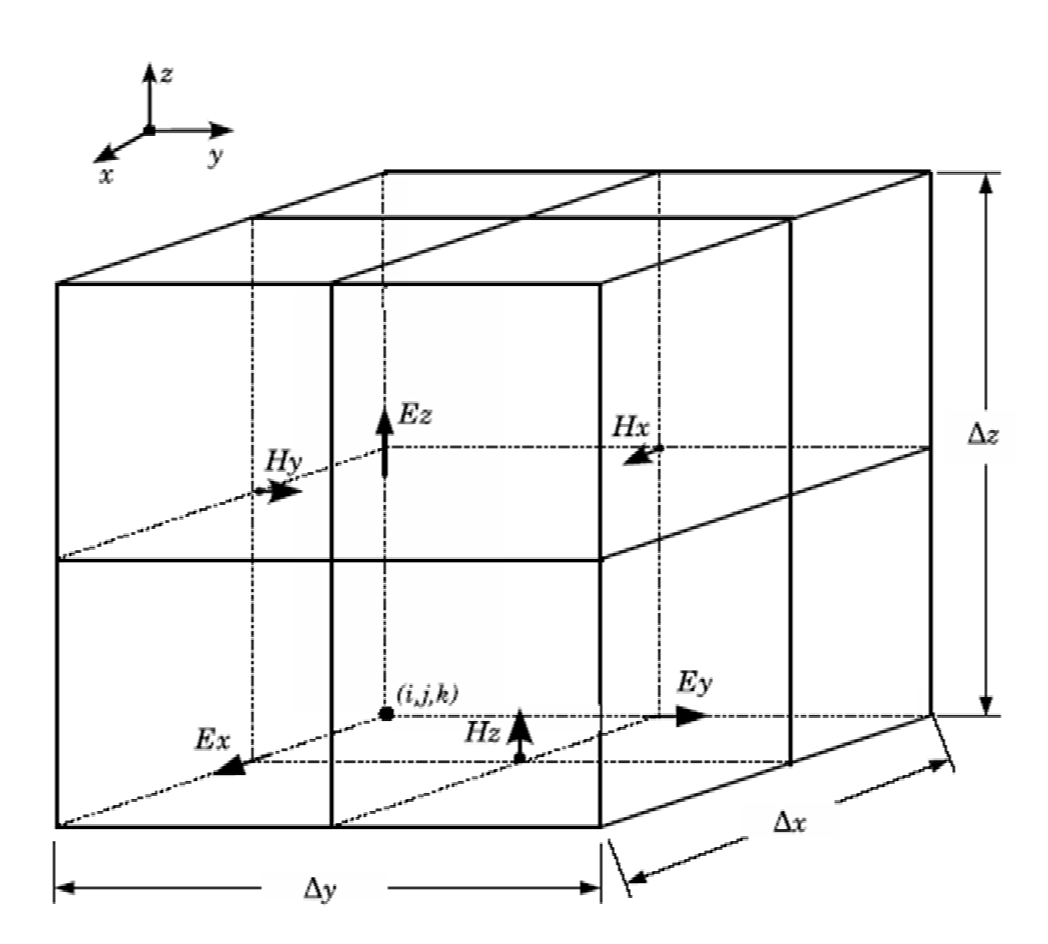
\includegraphics[scale=0.5]{celula}
	\caption{Célula Yee.}
	\label{fg:celulaYee}
\end{figure} 
		
Para que possam ser realizadas simulações de propagação de onda em FDTD, é criada uma malha 3D formada por múltiplas células de Yee que preenche toda região de análise, Figura\ref{fg:grade}\cite{almeida}, com a finalidade de mostrar as componentes de campo $\overline{E}$ e $\overline{H}$ atuantes em cada ponto da malha desta região.	\\
\begin{figure}[ht!]
	\centering
	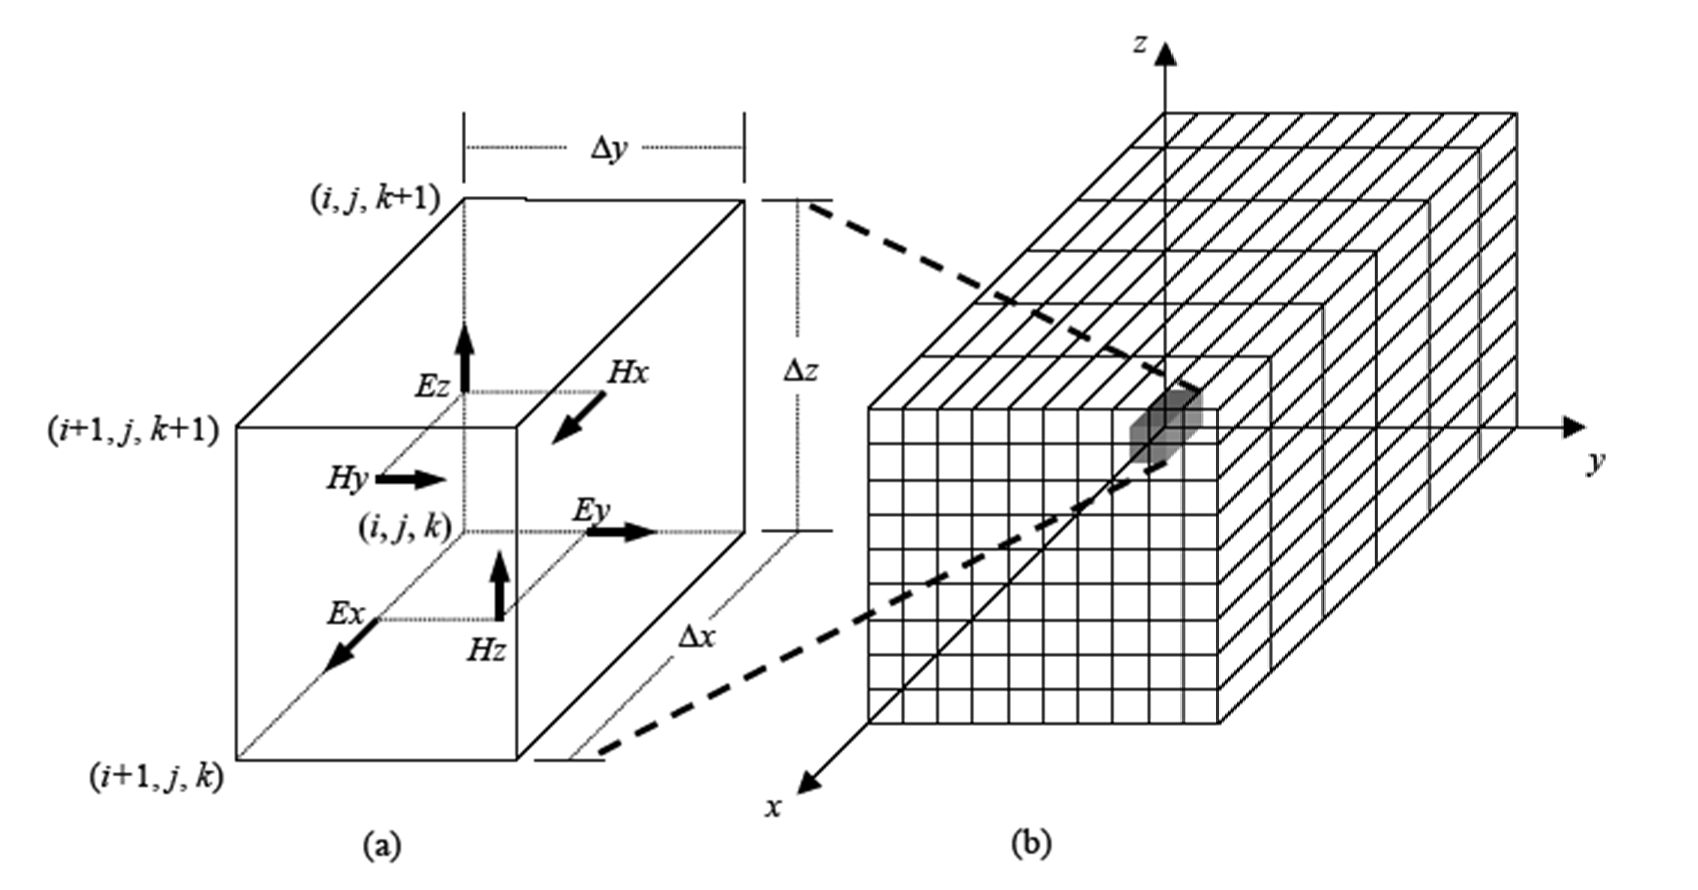
\includegraphics[scale=0.5]{Malha3D}
	\caption{(a) Posição das componentes dos campos elétrico e magnético em uma célula de Yee;(b) Célula no interior de uma malha 3-D.}
	\label{fg:grade}
\end{figure} 

A referência a cada célula que compõe a malha, assim com as suas respectivas componentes de campo, é feita de forma discreta pelos índices $i, j$ e $k$, de forma que uma determinada posição $x, y, z$ (em metros) é referenciada no espaço discreto por $i, j, k$ (número da célula correspondente). Estas  referências são obtidas através das relações $x = i.\Delta_x, y = j.\Delta_{y}$ e $z = k.\Delta_z$, onde  $\Delta_x,  \Delta_y$ e $\Delta_z$ são as dimensões das células de Yee(Figura\ref{fg:celulaYee}).
